% In your .tex file
% !TEX program = latex
%  A simple AAU report template.
%  2014-09-13 v. 1.1.0
%  Copyright 2010-2014 by Jesper Kjær Nielsen <jkn@es.aau.dk>
%
%  This is free software: you can redistribute it and/or modify
%  it under the terms of the GNU General Public License as published by
%  the Free Software Foundation, either version 3 of the License, or
%  (at your option) any later version.
%
%  This is distributed in the hope that it will be useful,
		%  but WITHOUT ANY WARRANTY; without even the implied warranty of
%  MERCHANTABILITY or FITNESS FOR A PARTICULAR PURPOSE.  See the
%  GNU General Public License for more details.
%
%  You can find the GNU General Public License at <http://www.gnu.org/licenses/>.
%
%  A simple AAU report template.
%  2014-09-13 v. 1.1.0
%  Copyright 2010-2014 by Jesper Kjær Nielsen <jkn@es.aau.dk>
%
%  This is free software: you can redistribute it and/or modify
%  it under the terms of the GNU General Public License as published by
%  the Free Software Foundation, either version 3 of the License, or
%  (at your option) any later version.
%
%  This is distributed in the hope that it will be useful,
%  but WITHOUT ANY WARRANTY; without even the implied warranty of
%  MERCHANTABILITY or FITNESS FOR A PARTICULAR PURPOSE.  See the
%  GNU General Public License for more details.
%
%  You can find the GNU General Public License at <http://www.gnu.org/licenses/>.
%
\documentclass[11pt,twoside,a4paper,openright]{memoir}
%%%%%%%%%%%%%%%%%%%%%%%%%%
%% COMMAND DEACTIVATION %%
%%%%%%%%%%%%%%%%%%%%%%%%%%

\let\added\undefined
\let\deleted\undefined


%%%%%%%%%%%%%%
%% PACKAGES %%
%%%%%%%%%%%%%%


%%% Initial things %%%
% Fix various issues with LaTeX2e
\usepackage{fixltx2e}
% Font package
\usepackage{fourier}
% Index
\usepackage{makeidx}
\makeindex


%%% Translations and character encodings %%%
% Enable use of several characters, including æ, ø and å
\usepackage[utf8]{inputenc}
%  language
\usepackage[english]{babel}
% Use PostScript fonts instead of bitmap ones. Also does other stuff.
\usepackage[T1]{fontenc}
% Various LaTeX symbols
\usepackage{latexsym}
% Wider selection of colours
\usepackage[pdftex,dvipsnames,table]{xcolor}  % Coloured text etc.% Improved element justification
\usepackage{ragged2e}
% Font improvements
\usepackage{fix-cm}
% Enables inclusion of PDF files
\usepackage{pdfpages}
% Enables various forms of lines, like double-underlining (\uuline{})
\usepackage[normalem,normalbf]{ulem}
% Sets the tolerance for distance between words, determining when to hyphenate.
\pretolerance=2500


%%% Figures and tables (Floats) %%%
% Ensures that floats won't appear -before- the place where they're added
\usepackage{flafter}
% Enable multi-rows and -columns
\usepackage{multirow}
\usepackage{multicol}
% Double, horizontal lines
\usepackage{hhline}
% Enables coloured tables
\usepackage{colortbl}
% Gives improved control over placement of floats
% \begin{figure}[!h] % Won't be floating
\usepackage{here}
% Wrap text around figures
\usepackage{wrapfig}
% Wrap text around tables
\usepackage{floatflt}
% Enables the \FloatBarrier command
\usepackage{placeins}
% Rotation of figures
\usepackage{rotating}
% Framed boxes
\usepackage{framed}
% Booktabs - Fancy tables
\usepackage{booktabs}
% Enables inclusion of PDF documents of version 1.6+
%\pdfoptionpdfminorversion=6


%%% Mathematic formulas %%%
% AMS math
%\usepackage{amsmath}
%\usepackage{amssymb}
% Extra fonts (for math, I think)
\usepackage{stmaryrd}
% Access text symbols
\usepackage{textcomp}
% Extend AMS
%\usepackage{mathtools}
%\usepackage{cancel}
% Use theorems in your document
% The ntheorem package is also used for the example environment
% When using thmmarks, amsmath must be an option as well. Otherwise \eqref doesn't work anymore.
%\usepackage[framed,amsmath,thmmarks]{ntheorem}
% Pretty fractions, just because
%\usepackage{nicefrac}


%%% Graphics %%%
% Various image-commands
\usepackage{eso-pic}
% Use JPEG and PNG images
\usepackage{array,graphicx}
\DeclareGraphicsExtensions{.pdf,.png,.jpg}
\graphicspath{{./images/}}
%Wrapping Images
\usepackage{wrapfig}


%%% Text stuff %%%
% Filler text
%\usepackage{lipsum}
% Page counting
%\usepackage{totpages}
% Acronyms
%\usepackage{acronym}
%avoid widows
%\widowpenalty10000


%%% Source Code Stuff %%%
% Adds \lstinline!code there!, where !! are delimeters not used in the code
% Adds the environment: lstlisting
% Adds command \lstinputlisting[options]{filename.ext}
% More info in manual.
%\usepackage{listings}
%\lstloadlanguages{[Sharp]C,XML,SQL}
%\lstset{numbers=left,
%        numberstyle=\tiny,
%        stepnumber=2,
%        numbersep=5pt,
%        frame=tb,
%        inputencoding=utf8,
%        tabsize=2,
%        extendedchars=true,
%        language=[Sharp]C}

\usepackage{color}
\definecolor{bluekeywords}{rgb}{0.13,0.13,1}
\definecolor{greencomments}{rgb}{0,0.5,0}
\definecolor{redstrings}{rgb}{0.9,0,0}

\usepackage{courier}

\usepackage{listings}

\lstdefinelanguage{JavaScript}{
  keywords={typeof, new, true, false, catch, function, return, null, catch, switch, var, if, in, while, do, else, case, break},
  keywordstyle=\color{blue}\bfseries,
  ndkeywords={class, export, boolean, throw, implements, import, this},
  ndkeywordstyle=\color{darkgray}\bfseries,
  identifierstyle=\color{black},
  sensitive=false,
  comment=[l]{//},
  morecomment=[s]{/*}{*/},
  commentstyle=\color{purple}\ttfamily,
  stringstyle=\color{red}\ttfamily,
  morestring=[b]',
  morestring=[b]"
}


\lstset{language=[Sharp]C,
  captionpos=b,            
  columns=fixed,     
  numbers=left,
  numberstyle=\tiny,
  showspaces=false,
  showtabs=false,
  breaklines=true,
  inputencoding=utf8,
  showstringspaces=false,
  breakatwhitespace=true,
  escapeinside={(*@}{@*)},
  commentstyle=\color{greencomments},
  keywordstyle=\color{bluekeywords},
  stringstyle=\color{redstrings},
  basicstyle=\ttfamily\small,
  literate={ø}{{\o}}1
  		   {æ}{{\ae}}1
  		   {å}{{\aa}}1
  		   {Ø}{{\O}}1
  		   {Æ}{{\AE}}1
  		   {Å}{{\AA}}1
         {§}{{\S}}1
}

\lstdefinestyle{make}{tabsize=4}

%%% References, bibtex and URLs %%%
% Post URLs. Allows breaking at hyphens to help avoid long links.
\usepackage[hyphens]{url}
% Better cross references
\usepackage[danish]{varioref}
% Enable natbib citation styles
\usepackage[numbers]{natbib}
% Define a new 'leo' style for URL package, that will use a smaller font
\makeatletter
\def\url@leostyle{%
  \@ifundefined{selectfont}{\def\UrlFont{\sf}}{\def\UrlFont{\small\ttfamily}}
}
\makeatother
% And of course, use this new style
\urlstyle{leo}




%%% Floats %%%
% Not entirely sure why I need this yet
\let\newfloat\relax
\usepackage{float}
% Enables usage of \subcaption, \subtop and \subbottom
\newsubfloat{figure}


%%% Todo Stuff %%%
% Insert needed corrections with \fixme{..}, which will cause an error during compile, if any are present once 'draft'
% is replaced with 'final'
\usepackage[footnote,draft,english,silent,nomargin]{fixme}
\fxsetup{layout={footnote,marginclue,index},innerlayout={inline,index}}


%%% Changes Markup %%%
% Markup changes of varying types.
% Adds the commands:
%  - \added[id=(author id), remark={remark text}]{new text}
%  - \deleted[id=(author id), remark={remark text}]{old text}
%  - \replaced[id=(author id), remark={remark text}]{new text}{old text}
\usepackage[xcolor,authormarkup=footnote]{changes}
% Adds the commands:
%  - \cbstart
%  - \cbend
%  - \cbdelete
%  - Environment: changebar
\usepackage[outerbars,xcolor]{changebar}
\cbcolor{red}



%%%%%%%%%%%%%%%%%%%%%%%
%% DOCUMENT SETTINGS %%
%%%%%%%%%%%%%%%%%%%%%%%


%%% Margins %%%
% \setlrmarginsandblock{binding}{edge}{ratio}
\setlrmarginsandblock{2.0cm}{2.0cm}{*}
% \setulmarginsandblock{top}{bottom}{ratio}
\setulmarginsandblock{2.0cm}{2.0cm}{*}
% Performs various calculations and makes several non-Memoir things work with the Memoir class
\checkandfixthelayout 
% Correct todonotes placement
\reversemarginpar


%%% Paragraph formatting %%%
% Size of paragraph indentation
\setlength{\parindent}{0mm}
% Distance between paragraphs (double enter)
\setlength{\parskip}{3mm}
% Line distance
\linespread{1,1}


%%% Bibliography %%%
% Defines parameters for the bibliography, such as the parenthesis and separators
%%%% OLD STYLE!
%\bibpunct{[}{]}{,}{a}{}{;}
% Bibliography style
%%%% OLD STYLE!
%\bibliographystyle{bibtex/harvard}
%\bibliographystyle{plainnat}
\bibliographystyle{unsrt}


%%% Table of contents %%%
% Depth of numbered headlines
\setsecnumdepth{subsubsection}
% Changing the document class' limit for number-depth
\maxsecnumdepth{subsection}
% Define the depth included in the table of contents
\settocdepth{section}
% Use letters instead of Roman numerals in TOC
\renewcommand{\thepart}{\Alph{part}}


%%% Text stuff %%%
% Removes distance between items in itemize
%\let\olditemize=\itemize
%\def\itemize{\olditemize\setlength{\itemsep}{-1ex}}
%% Removes distance between items in enumerate
%\let\oldenumerate=\enumerate
%\def\enumerate{\oldenumerate\setlength{\itemsep}{-1ex}}
\usepackage{enumitem}


%%% Changes (Language strings) %%%
\addto\captionsdanish{
  \def\listofchangesname{Ændringer i dokumentet}
  \def\summaryofchangesname{Ændringer}
  \def\changesaddname{Tilføjet}
  \def\changesdeletename{Slettet}
  \def\changesreplacename{Erstattet}
  \def\changesauthorname{Skribent}
  \def\changesanonymousname{anonym}
  \def\changesnoloc{Listen af ændringer tilgængelig efter næste \LaTeX\ kørsel.}
  \def\changesnosoc{Opsummering af ændringer tilgængelig efter næste \LaTeX\ kørsel.}
}


%%% Visual references %%%
% Enables clickable hyperlinks

%%% Add hidelinks to remove boxes around links

\usepackage[colorlinks,backref=page]{hyperref}
% General setup of hyperlinks package
\hypersetup{
    breaklinks = true,
    colorlinks = false,
    linkcolor = black,
    anchorcolor = black,
    citecolor = black
}


%%% Colour definitions %%%
% Defines: gray
\definecolor{gray}{gray}{0.80}
% Defines: numbercolor
\definecolor{numbercolor}{gray}{0.7}
% Defines: shadecolor
\definecolor{shadecolor}{RGB}{33,26,82}
% Defines: aaublue
\definecolor{aaublue}{RGB}{33,26,82}


%%% Figure and table texts setup %%%
% Font definition for the 'Figure' or 'Table' displays.
\captionnamefont{\small\bfseries\itshape}
% Font definition for the numbering
\captiontitlefont{\small}
% Delimiter between number and figure text
\captiondelim{. }
% Left justify multi-line figure texts below one another
\hangcaption
% Width of figure text
\captionwidth{\linewidth}
% Distance below figure text
\setlength{\belowcaptionskip}{10pt}
% Fix space between figure number and name
\setlength{\cftfigurenumwidth}{14mm}


%%% Page header and footer %%%
% Define width of header and footer
\setlength{\headwidth}{\textwidth}
% Create pagestyle for pages with and without a new chapter
\makepagestyle{reportPlain}
\makepagestyle{reportChapter}
% Pagestyle for chapter pages (Only a footer, of course)
\makefootrule{reportChapter}{\headwidth}{\normalrulethickness}{\footruleskip}
\makeevenfoot{reportChapter}{\thepage}{}{}
\makeoddfoot{reportChapter}{}{}{\thepage}
% Pagestyle for regular pages
\makerunningwidth{reportPlain}{\headwidth}
\makeheadposition{reportPlain}{flushright}{flushleft}{flushright}{flushleft}
\makeevenhead{reportPlain}{\leftmark}{}{}
\makeoddhead{reportPlain}{}{}{\rightmark}
\makeevenfoot{reportPlain}{\thepage}{}{}
\makeoddfoot{reportPlain}{}{}{\thepage}
\makeheadrule{reportPlain}{\headwidth}{\normalrulethickness}
\makefootrule{reportPlain}{\headwidth}{\normalrulethickness}{\footruleskip}
% Use pagestyles
\pagestyle{reportPlain}
\aliaspagestyle{chapter}{reportChapter}
\aliaspagestyle{part}{reportChapter}
\aliaspagestyle{title}{empty}
% Do not stretch pages
\raggedbottom


%%% Naming %%%
% Define various names for captions and such
%\addto\captionsdanish{
 % \renewcommand\appendixname{Bilag}
%  \renewcommand\contentsname{Indholdsfortegnelse} 
%  \renewcommand\appendixpagename{Bilag}
%  \renewcommand\cftchaptername{\chaptername~}
%  \renewcommand\cftappendixname{\appendixname~}
%  \renewcommand\appendixtocname{Bilag}
%}


%%% Appendix setup %%%
% Appendix setup. Might need some settings here
\usepackage{appendix}


%%% Chapter look and feel %%%
% Define style: jenor
\newif\ifchapternonum
\makechapterstyle{jenor}{
  \renewcommand\printchaptername{}
  \renewcommand\printchapternum{}
  \renewcommand\printchapternonum{\chapternonumtrue}
  \renewcommand\chaptitlefont{\fontfamily{pbk}\fontseries{db}\fontshape{n}\fontsize{25}{35}\selectfont\raggedleft}
  \renewcommand\chapnumfont{\fontfamily{pbk}\fontseries{m}\fontshape{n}\fontsize{1in}{0in}\selectfont\color{numbercolor}}
  \renewcommand\printchaptertitle[1]{%
    \noindent
    \ifchapternonum
    \begin{tabularx}{\textwidth}{X}
    {\let\\\newline\chaptitlefont ##1\par}
    \end{tabularx}
    \par\vskip-2.5mm\hrule
    \else
    \begin{tabularx}{\textwidth}{Xl}
    {\parbox[b]{\linewidth}{\chaptitlefont ##1}} & \raisebox{-15pt}{\chapnumfont \thechapter}
    \end{tabularx}
    \par\vskip2mm\hrule
    \fi
  }
}
% Use style: jenor
%\chapterstyle{jenor}
\usepackage{titlesec, blindtext}
\definecolor{gray75}{gray}{0.75}
\newcommand{\hsp}{\hspace{20pt}}
\titleformat{\chapter}[hang]{\Huge\bfseries\vspace{-40pt}}{\thechapter\vspace{-20pt}\hsp\textcolor{gray75}{|}\hsp}{0pt}{\Huge\bfseries\vspace{-20pt}}

%%% Misc stuff %%%
% Use regular numbers for pages
%\pagenumbering{arabic}
% Word and letter counts
\newcommand{\wordcount}{\input{preamble/sums/wordcount.sum}}
\newcommand{\charcount}{\input{preamble/sums/charcount.sum}}
\newcommand{\lettercount}{\charcount}
\newif\ifcounts
% Italicized quote-environment
\newenvironment{italicquote}{\begin{quote}\itshape}{\end{quote}}
% Acronyms in list or not (true if in list)
\newif\ifAcroList
\AcroListfalse


%%% Left-aligning bibliography %%%
%\renewcommand*{\bibfont}{\raggedright}


%%%% these patches ensure that the backrefs point to the actual occurrences of the citations in the text, not just the page or section in which they appeared
%%%% http://tex.stackexchange.com/questions/54541/precise-back-reference-target-with-hyperref-and-backref
%%%% BEGIN BACKREF DIRECT PATCH, apply these AFTER loading hyperref package with appropriate backref option
% The following options are provided for the patch, currently with a poor interface!
% * If there are multiple cites on the same (page|section) (depending on backref mode),
%   should we show only the first one or should we show them all?
\newif\ifbackrefshowonlyfirst
\backrefshowonlyfirstfalse
%\backrefshowonlyfirsttrue
%%%% end of options
%
% hyperref is essential for this patch to make any sense, so it is not unreasonable to request it be loaded before applying the patch
\makeatletter
% 1. insert a phantomsection before every cite, so hyperref has something to target
%    * in case natbib is loaded. hyperref provides an appropriate hook so this should be safe, and we don't even need to check if natbib is loaded!
\let\BR@direct@old@hyper@natlinkstart\hyper@natlinkstart
\renewcommand*{\hyper@natlinkstart}{\phantomsection\BR@direct@old@hyper@natlinkstart}% note that the anchor will appear after any brackets at the start of the citation, but that's not really a big issue?
%    * if natbib isn't used, backref lets \@citex to \BR@citex during \AtBeginDocument
%      so just patch \BR@citex
\let\BR@direct@oldBR@citex\BR@citex
\renewcommand*{\BR@citex}{\phantomsection\BR@direct@oldBR@citex}%

% 2. if using page numbers, show the page number but still hyperlink to the phantomsection instead of just the page!
\long\def\hyper@page@BR@direct@ref#1#2#3{\textit{\hyperlink{#3}{Page #1}}}

% check which package option the user loaded (pages (hyperpageref) or sections (hyperref)?)
\ifx\backrefxxx\hyper@page@backref
    % they wanted pages! make sure they get our re-definition
    \let\backrefxxx\hyper@page@BR@direct@ref
    \ifbackrefshowonlyfirst
        %\let\backrefxxxdupe\hyper@page@backref% test only the page number
        \newcommand*{\backrefxxxdupe}[3]{#1}% test only the page number
    \fi
\else
    \ifbackrefshowonlyfirst
        \newcommand*{\backrefxxxdupe}[3]{#2}% test only the section name
    \fi
\fi

% 3. now make sure that even if there is no numbered section, the hyperref's still work instead of going to the start of the document!
\RequirePackage{etoolbox}
\patchcmd{\Hy@backout}{Doc-Start}{\@currentHref}{}{\errmessage{I can't seem to patch backref}}
\makeatother
%%%% END BACKREF PATCHES


% Enable figures like checkmarks
\usepackage{pifont}
\newcommand{\cmark}{\ding{51}}%
\newcommand{\xmark}{\ding{55}}%

%%%%%%%%%%%%%%%%%%%%%%%%%%%%%%%%%%%%%%%%%%%%%%%%
%Flowchart
\usepackage{tikz}
\usetikzlibrary{shapes.geometric, arrows, positioning, matrix, automata, positioning}
%%%%%%%%%%%%%%%%%%%%%%%%%%%%%%%%%%%%%%%%%%%%%%%%

%\usepackage{bera}% optional: just to have a nice mono-spaced font

\newcommand*\rot{\rotatebox{90}}

\colorlet{punct}{red!60!black}
\definecolor{background}{HTML}{EEEEEE}
\definecolor{delim}{RGB}{20,105,176}
\colorlet{numb}{magenta!60!black}

\lstdefinelanguage{json}{
    basicstyle=\normalfont\ttfamily,
    numbers=left,
    numberstyle=\scriptsize,
    stepnumber=1,
    numbersep=8pt,
    showstringspaces=false,
    breaklines=true,
    frame=lines,
    backgroundcolor=\color{background},
    literate=
     *{:}{{{\color{punct}{:}}}}{1}
      {,}{{{\color{punct}{,}}}}{1}
      {\{}{{{\color{delim}{\{}}}}{1}
      {\}}{{{\color{delim}{\}}}}}{1}
      {[}{{{\color{delim}{[}}}}{1}
      {]}{{{\color{delim}{]}}}}{1},
}


%% SOME MACROS HYPE

\newcommand{\class}[1] {\texttt{#1}}


%%%%%%%%%%%%%%%%%%%%%%%%%%%%%%%%%%%%%%%%%%%%%%%%
% Misc
%%%%%%%%%%%%%%%%%%%%%%%%%%%%%%%%%%%%%%%%%%%%%%%%
% Add bibliography and index to the table of
% contents
% Add the command \pageref{LastPage} which refers to the
% page number of the last page
%\usepackage[
% disable, %turn off todonotes
%colorinlistoftodos, %enable a coloured square in the list of todos
%textwidth=\marginparwidth, %set the width of the todonotes
%textsize=scriptsize, %size of the text in the todonotes
%prependcaption
%]{todonotes}
%\usepackage{xargs}                      % Use more than one optional parameter in a new commands

\usepackage{tocbibind}

\usepackage[english]{cleveref}
\crefname{exa}{eksempel}{eksempler}
\newcommand{\myref}[1]{\Cref{#1}}
\newcommand{\Myref}[1]{\Cref{#1}}
\newcommand{\lowercaseref}[1]{\cref{#1}}

\def\sectionautorefname{Section}

% GLOSARIEIASI
\usepackage[acronym]{glossaries}
\usepackage{xparse}

\makeglossaries

%\newglossaryentry{gpu}{name=GPU, description={Graphics Processing Unit}}
%\newglossaryentry{cpu}{name=CPU, description={Central Processing Unit}}
%\newglossaryentry{gpgpu}{name=GPGPU, description={General-Purpose computing on Graphics Processing Units}}

% \gls{CUDA}
% \glspl{CUDAs}
% \Gls{<label>}
\newglossaryentry{cuda}{name=CUDA, description={Compute Unified Device Architecture: a parallel computing platform and programming model created by NVIDIA.}}
\newglossaryentry{gamble}{name=GAMBL, description={The name of the programming language made in this report.}}
\newglossaryentry{opencl}{name=OpenCL, description={Open Computing Language: a framework for writing programs that execute across heterogeneous platforms.}}
\newglossaryentry{heterogeneous}{name=heterogeneous, description={Systems with more than one kind of processor can be described as a heterogenous system.}}
\newglossaryentry{Parallel Thread Execution}{name=PTX, description={Pseudo-assembly languange used by Nvidia and OpenCL as the target languange when compiling kernals}}

% \acrfull == CentralProcessingUnit(CPU)
% \acrlong == CentralProcessingUnit
% \acrshort == CPU
\newacronym{cpu}{CPU}{Central Processing Unit}
\newacronym{gpu}{GPU}{Graphics Processing Unit}
\newacronym{gpgpu}{GPGPU}{General-Purpose computing on Graphics Processing Units}
\newacronym{simd}{SIMD}{Single Instruction Multiple Data}
\newacronym{ebnf}{EBNF}{Extended Backus–Naur Form}
\newacronym{cfg}{CFG}{Context-Free Grammar}
\newacronym{regex}{regex}{regular expression}
\newacronym{ast}{AST}{Abstract Syntax Tree}
\newacronym{antlr}{ANTLR}{ANother Tool for Languange Recognition}
\newacronym{jit}{JIT}{Just-In-Time}
\newacronym{ptx}{PTX}{Parallel Thread Execution}


\usepackage{xargs}                      % Use more than one optional parameter in a new commands
\usepackage[colorinlistoftodos,prependcaption,textsize=tiny]{todonotes}

%\usepackage[colorinlistoftodos,prependcaption,textsize=tiny]{todonotes}
\newcommandx{\unsure}[2][1=]{\todo[linecolor=red,backgroundcolor=red!25,bordercolor=red,#1]{#2}}
\newcommandx{\change}[2][1=]{\todo[linecolor=blue,backgroundcolor=blue!25,bordercolor=blue,#1]{#2}}
\newcommandx{\info}[2][1=]{\todo[linecolor=OliveGreen,backgroundcolor=OliveGreen!25,bordercolor=OliveGreen,#1]{#2}}
\newcommandx{\improvement}[2][1=]{\todo[linecolor=Plum,backgroundcolor=Plum!25,bordercolor=Plum,#1]{#2}}
\newcommandx{\thiswillnotshow}[2][1=]{\todo[disable,#1]{#2}}



\usepackage{tikz}

\usetikzlibrary{shapes.geometric, arrows}

\tikzstyle{lille} = [rectangle, minimum width=2cm, minimum height=1cm,text centered, draw=black, fill=blue!30]
\tikzstyle{main} = [rectangle, minimum width=2cm, minimum height=2cm,text centered, draw=black, fill=red!30]
\tikzstyle{hoj} = [rectangle, minimum width=1cm, minimum height=2cm,text centered, draw=black, fill=red!30]
\tikzstyle{cloud} = [draw, ellipse,fill=yellow!20, node distance=0.7cm, minimum height=2em]
\tikzstyle{invi} = [draw, ellipse, node distance=3cm, minimum height=2em]
\tikzstyle{line} = [draw, -latex']
\tikzstyle{arrow} = [thick,->,>=stealth]
\tikzstyle{blockz} = [rectangle, minimum width=4cm, minimum height=1cm,text centered, draw=black, fill=blue!30]




\usepackage{pdflscape}% package inclusion and set up of the document
% see, e.g., http://en.wikibooks.org/wiki/LaTeX/Formatting#Hyphenation
% for more information on word hyphenation
\hyphenation{ex-am-ple hy-phen-a-tion short}
\hyphenation{long la-tex}
% 
%  A simple AAU report template.
%  2014-09-13 v. 1.1.0
%  Copyright 2010-2014 by Jesper Kjær Nielsen <jkn@es.aau.dk>
%
%  This is free software: you can redistribute it and/or modify
%  it under the terms of the GNU General Public License as published by
%  the Free Software Foundation, either version 3 of the License, or
%  (at your option) any later version.
%
%  This is distributed in the hope that it will be useful,
%  but WITHOUT ANY WARRANTY; without even the implied warranty of
%  MERCHANTABILITY or FITNESS FOR A PARTICULAR PURPOSE.  See the
%  GNU General Public License for more details.
%
%  You can find the GNU General Public License at <http://www.gnu.org/licenses/>.
%
%
%
% see, e.g., http://en.wikibooks.org/wiki/LaTeX/Customizing_LaTeX#New_commands
% for more information on how to create macros

%%%%%%%%%%%%%%%%%%%%%%%%%%%%%%%%%%%%%%%%%%%%%%%%
% Macros for the titlepage
%%%%%%%%%%%%%%%%%%%%%%%%%%%%%%%%%%%%%%%%%%%%%%%%
%Creates the aau titlepage
\newcommand{\aautitlepage}[3]{%
  {
    %set up various length
    \ifx\titlepageleftcolumnwidth\undefined
      \newlength{\titlepageleftcolumnwidth}
      \newlength{\titlepagerightcolumnwidth}
    \fi
    \setlength{\titlepageleftcolumnwidth}{0.5\textwidth-\tabcolsep}
    \setlength{\titlepagerightcolumnwidth}{\textwidth-2\tabcolsep-\titlepageleftcolumnwidth}
    %create title page
    \thispagestyle{empty}
    \noindent%
    \begin{tabular}{@{}ll@{}}
      \parbox{\titlepageleftcolumnwidth}{
        \iflanguage{danish}{%
          
\includegraphics[width=\titlepageleftcolumnwidth]{figures/aau_logo_da}
        }{%
          
\includegraphics[width=\titlepageleftcolumnwidth]{figures/aau_logo_en}
        }
      } &
      \bigskip\\
       #1 &
      \parbox[t]{\titlepagerightcolumnwidth}{%
      \textbf{Abstract:}\bigskip\par
        \fbox{\parbox{\titlepagerightcolumnwidth-2\fboxsep-2\fboxrule}{%
          #3
        }}
      }\\
    \end{tabular}
    \vfill
    \iflanguage{danish}{%
      \noindent{\footnotesize\emph{Rapportens indhold er frit tilgængeligt, men offentliggørelse (med kildeangivelse) må kun ske efter aftale med forfatterne.}}
    }{%
      \noindent{\footnotesize\emph{The content of this report is freely available, but publication (with reference) may only be pursued due to agreement with the author.}}
    }
    \clearpage
  }
}

%Create english project info
\newcommand{\englishprojectinfo}[8]{%
  \parbox[t]{\titlepageleftcolumnwidth}{
    \textbf{Title:}\\ #1\bigskip\par
    \textbf{Theme:}\\ #2\bigskip\par
    \textbf{Project Period:}\\ #3\bigskip\par
    \textbf{Project Group:}\\ #4\bigskip\par
    \textbf{Participant(s):}\\ #5\bigskip\par
    \textbf{Supervisor(s):}\\ #6\bigskip\par
    \textbf{Copies:} #7\bigskip\par
    \textbf{Number of pages:} \pageref{LastPage}
    \bigskip\par
    \textbf{Date of Completion:}\\ #8
  }
}

%Create danish project info
\newcommand{\danishprojectinfo}[8]{%
  \parbox[t]{\titlepageleftcolumnwidth}{
    \textbf{Titel:}\\ #1\bigskip\par
    \textbf{Tema:}\\ #2\bigskip\par
    \textbf{Projektperiode:}\\ #3\bigskip\par
    \textbf{Projektgruppe:}\\ #4\bigskip\par
    \textbf{Deltager(e):}\\ #5\bigskip\par
    \textbf{Vejleder(e):}\\ #6\bigskip\par
    \textbf{Oplagstal:} #7\bigskip\par
    \textbf{Sidetal:} %\pageref{LastPage}
    \bigskip\par
    \textbf{Afleveringsdato:}\\ #8
  }
}
% my new macros

\begin{document}
%frontmatter
\pagestyle{empty} %disable headers and footers
\pagenumbering{roman} %use roman page numbering in the frontmatter
%  A simple AAU report template.
%  2014-09-13 v. 1.1.0
%  Copyright 2010-2014 by Jesper Kjær Nielsen <jkn@es.aau.dk>
%
%  This is free software: you can redistribute it and/or modify
%  it under the terms of the GNU General Public License as published by
%  the Free Software Foundation, either version 3 of the License, or
%  (at your option) any later version.
%
%  This is distributed in the hope that it will be useful,
%  but WITHOUT ANY WARRANTY; without even the implied warranty of
%  MERCHANTABILITY or FITNESS FOR A PARTICULAR PURPOSE.  See the
%  GNU General Public License for more details.
%
%  You can find the GNU General Public License at <http://www.gnu.org/licenses/>.
%
\pdfbookmark[0]{Front page}{label:frontpage}%
\thispagestyle{empty}
  \addtolength{\hoffset}{0.5\evensidemargin-0.5\oddsidemargin} %set equal margins on the frontpage - remove this line if you want default margins
  \noindent%
  \begin{tabular}{@{}p{\textwidth}@{}}
    \toprule[2pt]
    \midrule
    \vspace{0.2cm}
    \begin{center}
    \Huge{\textbf{
      GPU programming language% insert your title here
    }}
    \end{center}
    \begin{center}
      \Large{
        - A language to seemlessly take advange of the GPU -% insert your subtitle here
      }
    \end{center}
    \vspace{0.2cm}\\
    \midrule
    \toprule[2pt]
  \end{tabular}
  \vspace{4 cm}
  \begin{center}
    {\large
      Project Report%Insert document type (e.g., Project Report)
    }\\
    \vspace{0.2cm}
    {\Large
      SW413F15%Insert your group name or real names here
    }
  \end{center}
  \vfill
  \begin{center}
  Aalborg University\\
  Department of Computer Science
  \end{center}
\clearpage

\thispagestyle{empty}
{\small
\strut\vfill % push the content to the bottom of the page
\noindent Copyright \copyright{} Aalborg University 2014\par
\vspace{0.2cm}
\noindent Here you can write something about which tools and software you have used for typesetting the document, running simulations and creating figures. If you do not know what to write, either leave this page blank or have a look at the colophon in some of your books.
}
\clearpage


\pdfbookmark[0]{English title page}{label:titlepage_en}
\aautitlepage{%
  \englishprojectinfo{
    Project Title %title
  }{%
    Scientific Theme %theme
  }{%
    Fall Semester 2010 %project period
  }{%
    XXX % project group
  }{%
    %list of group members
    Author 1\\ 
    Author 2\\
    Author 3
  }{%
    %list of supervisors
    Supervisor 1\\
    Supervisor 2
  }{%
    1 % number of printed copies
  }{%
    \today % date of completion
  }%
}{%department and address
  \textbf{Electronics and IT}\\
  Aalborg University\\
  \href{http://www.aau.dk}{http://www.aau.dk}
}{% the abstract
  Here is the abstract
}

\cleardoublepage
{\selectlanguage{danish}
\pdfbookmark[0]{Danish title page}{label:titlepage_da}
\aautitlepage{%
  \danishprojectinfo{
    Rapportens titel %title
  }{%
    Semestertema %theme
  }{%
    Efterårssemestret 2010 %project period
  }{%
    XXX % project group
  }{%
    %list of group members
    Forfatter 1\\ 
    Forfatter 2\\
    Forfatter 3
  }{%
    %list of supervisors
    Vejleder 1\\
    Vejleder 2
  }{%
    1 % number of printed copies
  }{%
    \today % date of completion
  }%
}{%department and address
  \textbf{Elektronik og IT}\\
  Aalborg Universitet\\
  \href{http://www.aau.dk}{http://www.aau.dk}
}{% the abstract
  Her er resuméet
}}

\cleardoublepage
\pdfbookmark[0]{Contents}{label:contents}
\pagestyle{empty} %enable headers and footers again
\tableofcontents*
\listoftodos
\chapter*{Preface\markboth{Preface}{Preface}}\label{ch:preface}
\addcontentsline{toc}{chapter}{Preface}
Here is the preface. You should put your signatures at the end of the preface.

\vspace{\baselineskip}\hfill Aalborg University, \today
\vfill\noindent
\begin{minipage}[b]{0.45\textwidth}
 \centering
 \rule{\textwidth}{0.5pt}\\
  Author 1\\
 {\footnotesize <username1@XX.aau.dk>}
\end{minipage}
\hfill
\begin{minipage}[b]{0.45\textwidth}
 \centering
 \rule{\textwidth}{0.5pt}\\
  Author 2\\
 {\footnotesize <username2@XX.aau.dk>}
\end{minipage}
\vspace{3\baselineskip}
\begin{center}
\begin{minipage}[b]{0.45\textwidth}
 \centering
 \rule{\textwidth}{0.5pt}
  Author 3\\
 {\footnotesize <username3@XX.aau.dk>}
\end{minipage}
\end{center}

\cleardoublepage
%mainmatter
\pagenumbering{arabic}

\chapter{Introduction}\label{ch:introduction}

This paper is written by a group of Software Engineering students at Aalborg University.

Large Numerical computations has become possible to calculate faster on modern CPUs due to their enormous development of speed. 
However, a trend is starting to show, Moore's law will not continue as it has been doing for the past decades.
By 2022 it might stop being possible to make the transistor densities smaller, and by this time they should be around 7-5nms.\citep{Moore2013}


So if our processors are reaching their maximum potential, is it possible to use other kind of computational devices for these kind of tasks?

GPUs are extremely fast at calculating lots of data due to their internal architecture(More on this in chapter\todo{Marks kapitel}).
They are starting to be used around the world for calculating very large numerical computations, since it is possible to parallelize tasks on the GPUs much more than is possible on a CPU.
Most compilers like GCC, compiles for computations on the CPU, and it can be difficult to transfer these computations to the gpu instead using languages like C, or C++.
To do this, you can use CUDA or OpenCL.
CUDA is a programming model created by Nvidia, and is therefore only usable by CUDA enabled Nvidia GPUs.
OpenCL though is usable for more GPUs, like AMD, but Nvidia has stopped support for the newer versions of OpenCL(More on OpenCl and CUDA in chapter \todo{Mortens kapitel})
Therefore this project paper will research the possibilities of creating a programming language, and a compiler, which can perform numerical computations on the GPU seamlessly to the programmer. 
%METADATA about GPU, purpose and general difference from CPU
\section{Graphics Processing Units}
Graphic Processing Units (GPUs) were initially used to accelerate memory-intensive work for rendering graphics.
They consist of a higher amount of cores, these cores while each less powerfull than the cores used in a CPU, are so plentiful that with enough work, more data can be processed in paralell.
These cores sacrifice the architectural components that enables the CPU run single instruction streams in exchange for more computing power, such as increasing the number of \textbf{Arithmetic Logic Units (ALUs)} \myref{image:GPUCPUimage} shows a basic idea of the difference between the GPU and CPU. %http://pdsgroup.hpclab.ceid.upatras.gr/files/CUDA-Parallel-Computing-on-GPUs.pdf
\begin{figure}[h!]
\centering
 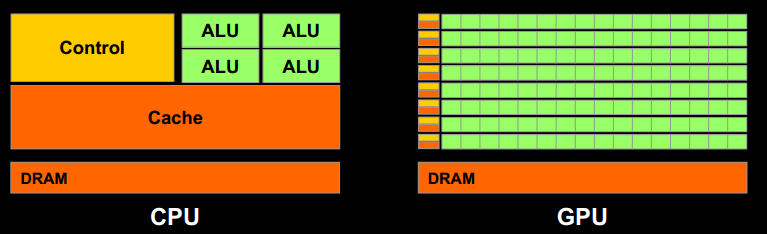
\includegraphics[width=1\textwidth]{figures/GPUCPUimage.png} % trim=4.85cm 15cm 0.85cm 1cm
\caption{A basic representation of the Transistor allocation on a GPU compared to a CPU}\label{image:GPUCPUimage} %ftp://download.nvidia.com/developer/cuda/seminar/TDCI_Arch.pdf
\vspace{-25pt}
\end{figure}

This concept of using many cores to process a high number of threads gives GPUs a high throughput, and is therefore a main principal of GPUs.
In recent years GPUs have been used for more than just graphical purposes, such as GPU-accelerated computing, the use of both GPU and CPU to accelerate scientific and analytical applications.
%http://www.nvidia.com/object/what-is-gpu-computing.html



%GPU Architecture
\subsection{GPU architecture}
For the purpose of this section it is worth noting that depending on the GPU manufacturer and the series of the GPU, the exact architecture may vary.
This section will therefore describe the architecture in a conceptual manor, and not go into specifics. 
Also note that the main difference between earlier and later models of the same manufacturer, is primarily size of memory, not the architectural concepts themselves.
The GPU architecture chosen as the basis for the following section is NVIDIA. 
They are the market share leader, discounting integrated graphics solutions. 
	%Kernels
	%SingleInstructionMultipleData (SIMD)
The GPU consists of compute units (\textbf{Streaming Multiprocessors (SMs)}) which each consists of processing elements (\textbf{Streaming Processors (SPs)}), registers, execution cores for integer and floating point operations as well as several caches; shared memory, texture memory and constant memory cache.
%http://www.cudahandbook.com/uploads/Chapter_8._Streaming_Multiprocessors.pdf
For GPU-accelerated computing the GPU acts as a co-processor for data which can be calculated in paralell.
The GPU is controlled by the CPU.
The CPU calls the GPU driver and starts a data transfer with the GPU or a \textbf{kernel} launch on the GPU.
A kernel is a function executed on the GPU. %, this is explained further on \myref{sec:opencl}.
A kernel specifies the number of threads and data it requires.
%http://www.cs.virginia.edu/~skadron/Papers/thesis_prateeksha.pdf
%GPU Memory Hierachy
\subsection{Memory Hierachy}
	%Register (per-SM, allocated to threads as specified - fastest and most plentiful)	
	%Local memory (SM holds local variables that cannot be computed at compile time) texture cache
	%Global (GPU) Visible to all threads of a kernel, resides in DRAM 
	%Constant memory (GPU) Each SM contains a small latency optimized cache for purpose of reading this memory DRAM
	%Shared memory (per-SM, shared amongst threads of a block) Seperate adress space
	%Host memory (CPU)

%http://www.cudahandbook.com/uploads/Chapter_8._Streaming_Multiprocessors.pdf
\begin{figure}[h!]
\centering
 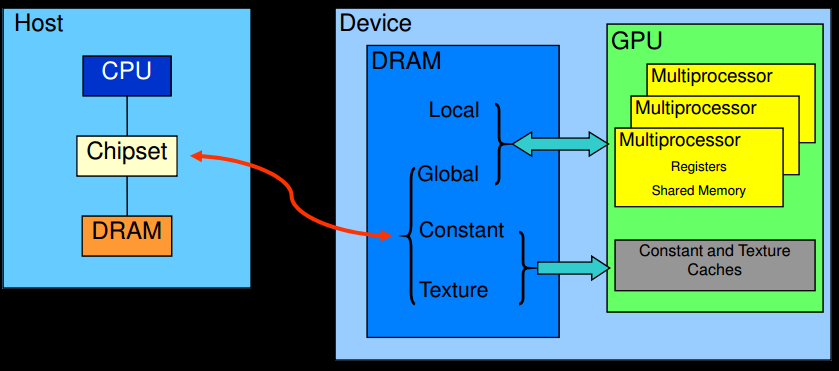
\includegraphics[width=1\textwidth]{figures/GPUMemoryClear.png} % trim=4.85cm 15cm 0.85cm 1cm
\caption{A basic representation of GPU memory hierarchy}\label{image:GPUMemory} 
\end{figure}
The GPU memory is comprised of the following different memory components, how it communicates is shown on \todo{OpenCLGPUMemoryModel}. 
Memory management of the GPU is also explicit, this means that the data must first be moved from the host, to global memory, then to local memory where the SMs can start to use it. 
Once they are done the result must be sent back the same way.
The memory architecture is designed with regard to performance by reducing memory traffic.
Although the hierarchy and its components were originally designed to improve performance for graphical applications, it can also be used efficiently in some GPU computing applications, how the memory is used is further explained in \todo{Advanced OpenCL}. %http://cuda-programming.blogspot.dk/2013/02/texture-memory-in-cuda-what-is-texture.html

\textbf{Registers:}

For any given SM, thousands of registers are contained, this is the most plentiful type of memory used in the SM. 
Once a kernel is launched, registers are allocated to threads as per the kernels requirements.
This also means that the registers are shared across the SM, but only to the allocated thread.
When allocated the registers are no longer available to the entire SM, once the thread is done and they can be reallocated.
The registers can each contain either integers and floating-points.

\textbf{Local Memory:}

Local memory is used for spilling registers as well as holding local variables.
Each SM has its own allocated local memory available which is available to the entire SM, unlike registers it is not controlled by the kernel being executed.

\textbf{Global and Constant Memory:}

The SMs can read and write to global memory, this is significantly slower than using local memory. %http://www.it.uu.se/edu/course/homepage/avdark/ht10/slides/09-GPU-and-OpenCL-4.pdf
Constant memory is read only for the SM however each SM contains a small optimized cache for the purpose of reading from this memory such that less reading is required. 
Both of these memory types are located on the DRAM and not in the SM.

\textbf{Shared Memory:}

Shared memory, as mentioned earlier, is part of the SM.
It is a very fast on-chip memory that threads can use for data interchange within thread blocks.
Although it is fast, being an on-chip per-SM resource, using it can affect the number of blocks and threads can used for computations.

\textbf{Texture Memory:}

Texture memory is shared amongst a number of SMs, like constant memory this is read-only for the SM and is cached in its own texture cache on the SM.

%Streaming Multiprocessors
\begin{wrapfigure}{r}{0.25\textwidth}
 \vspace{-50pt}
 \begin{center}
  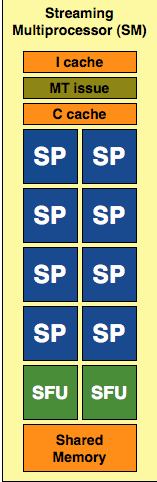
\includegraphics[width=0.23\textwidth]{figures/SM.png}
 \end{center}
 \caption{A basic representation of a SM.}\label{image:SM} 
 \vspace{-35pt}
\end{wrapfigure}
\subsection{Streaming Multiprocessors}
On the GPU the work is divided by the hardware.
When a kernel is launched, the hardware dynamically assign work groups to SMs, doing so while balancing the load across the GPU.
For each work group, a number of work items exists, these are the threads that execute the kernel.
Work items running on a SM can communicate through local memory, all the different work groups can communicate through global memory. %https://www.khronos.org/assets/uploads/developers/library/2009-hotchips/NVIDIA_OpenCL-for-NVIDIA-GPUs.pdf
A collection of a given number of SMs are refered to as a \textbf{Thread Processing Cluster (TPC)}, this TPC shares a controller, as well as a texture cache.
All SMs consist of a number of ALUs, \textbf{multiply-add (MAD)} and special function units for doing computations, multithreaded instruction fetch and issue unit, instruction cache, read-only constant cache and a shared memory cache, \myref{image:SM} shows an example of this, note that the ALUs and MAD corresponds to the SPs.
The SM schedules and executes threads in groups called warps.
A warp waits untill all its threads have finished execution, before the next instruction is fetched. 

%http://www.cs.virginia.edu/~skadron/Papers/thesis_prateeksha.pdf
\subsection{Conclusion} %This needs serious rework - but not now!
The architectural difference of the GPU from the CPU, are intented to maximize the throughput for problems that can handle a higher latency.
Such as an image, rather than the response time of a decive like a keyboard.
The lack of control and chache memory for the processing units used in the GPU, also greatly reduces its capabilities of handling complex issues that requires a concurrent apporach.
With the removal of such hardware as interrupts, an instruction in a given thread, will run till it is complete, and no thread will start without all the available ressource, as such given a complex problem stalls in the GPU would occur.
Thus some problems will be ill suited for the GPU but any problems that can be divided into smaller blocks of data and designated to run on different cores, will benefit substantially from the increased computing power the GPU provides.
The scheduling of said blocks are controlled by the hardware and as such no explicit management is required.
In conclusion due to the 10,000s threads available in a GPU, its memory hierachy for said threads and the hardwares ability to manage those threads, any problem that can be apporached with the SIMD model will be executed significantly faster than on any CPU.

%First Draft
%The result of this architecture is increased parallel computing power through the sacrifice of sequential computing power.
%The GPU sacrifices the cache memory of the CPU, in exchange for more computing power.
%This results in a very high throughput, work done in an amount of time, given that there is enough work.
%It also results in higher latency, the time from which an instruction is initiated untill the effects have taken place.
%Is is the direct opposite of a CPU.
%In a CPU low latency is preferred, the latency is hidden through its ability to do work concurrently the low latency is achieved by the caches, something which the GPU sacrificed.
%Although with low latency, also follows low throughput, which is why the GPU is more optimized for heavy computational work that can be done in parallel.
%The structure of SMs, and the work distribution of the GPU, is what enables it to use the SIMD model.
%The SM follows only one set of instructions but on multiple threads of data, the threads are managed and scheduled by the hardware itself.
%In conlusion, the GPU architecture allows us to efficiently compute any workload which can be done using parallel computing, and can tolerate the higher latency.

%GPU Results Parallel work/Multiprocessor programming
	%Latency/Throuhput optimizations and the result %label sec:comparch
\section{State of the art} % (fold)
\label{sec:state_of_the_art}
In this section different approaches to GPGPU using existing programming languages and libraries will be presented.
Each language and library will be running with either the OpenCL or the CUDA framework.
Every language and library described in this section can be found on \ref{tbl:sota} for an overview of their comparison.
      

\subsection{Libraries} 
There exists libraries for programming languages in order to utilise the GPU for computations by binding either to OpenCL or CUDA.
Generally the libraries used for GPU work often requires a lot of boilerplate and has what we deem to be a low level of abstraction.
The level of abstraction is based on how much control the programmer of the code has of the computer's resources.
I.e. if the programmer needs a line of code to allocate memory for each of the computations in the code, that results in low abstraction.
Boilerplate is the pieces of code which will have to be written with little to no alteration, in many different places of the code.
An example could be when making a call to a GPU, the boilerplate might be the code which handles this communication.
As an example we will look at C, Java and R, and some of their GPU Libraries.
Jcuda is a library for Java which support the use of CUDA, it has a lot of boilerplate, and low/medium abstraction level\citep{Java_library}. 
Jcuda requires many imports and the user needs to allocate a memory block for each element which causes the boilerplate code and the level of abstraction given.\citep{Java_malloc}
C has libraries such as CUDA C, OpenCL C and others.
These C libraries have the same problem as with the Java library as one needs to allocate memory for almost everything, and there is a lot of redundancy which creates a lot of boilerplate.
The abstraction level is therefore deemed low as one must keep in mind what is where and what can be done with each specific element.\citep{C_CUDA} 
There is also different libraries for the R language, one of which is called rpud.
It provides many functions from the R language, which can be performed on the GPU, and it is based on CUDA.
We deem that it has a high level of abstractions, since it is just function calls, without any memory allocation or direct GPU calls from the source code. \todo{Rcuda source}                                                 


\subsection{Theano (Python)}
Theano is a Python library that allows one to define, optimise, and evaluate mathematical expressions involving multi-dimensional arrays, while utilising the GPU.
The library has two ways of using the GPU; one with CUDA as back-end, and the other that should support any OpenCL compatible device as well NVIDIA cards.
The OpenCL implementation however does not support all the options available in the library due to an incomplete port of an old back-end.
While Theano supports CUDA and OpenCL, there is quite a bit of boilerplate and one must write different code in order to use either.
Theano does not require that the programmer allocates memory for arrays.
We deem that Theano has a medium level of abstraction since one has to declare if the GPU should be used and can only operate on single precision floats of 32 bits.
But on the other hand Theano does optimise the code by replacing methods with a GPU versions of the same methods to create transparency.\citep{Theano,Theano_GPU}

\subsection{MATLAB}
MATLAB is a high-level mathematical programming language with an interactive environment.
MATLAB supports the use of parallel computations in the form of using either a GPU or cloud computing.
It only natively supports the use of CUDA enabled NVIDIA GPUs for its parallel computations on GPUs, but OpenCL extensions do exist such that it becomes possible to use other devices.
The user of MATLAB much declare when the GPU must be used and also allocate memory for these tasks.
Declaring the memory gives a lot of boilerplate since it needs to be done for each element that one wants to compute.\citep{MATLAB_backend,MATLAB_benchmark}
Using the interactive environment provided by MATLAB there are built in tools for parallel computations on GPUs.
These tools provide a higher level of abstraction such as parallel for-loops (parfor) and special array types for distributed processing.
For GPU computing MATLAB simplify parallel code development by abstracting away the complexity of managing computations and data.\citep{MATLAB_parallel}

\subsection{Julia}
Julia is a high-level, high-performance dynamic programming language for technical computing, with syntax familiar to users of other technical computing environments.
The language supports C function calls directly with no use of wrappers or special APIs.
There are powerful shell-like capabilities for managing other processes.
Julia is designed for parallelism and cloud computing; making it efficient and easy to use.
Julia has a high level of abstraction because the user only needs a single keyword (\@parallel) for it to do the calculation in parallel.
The code is therefore looking clean without any boilerplate and is easy to read.
Julia uses both OpenCL and CUDA as back-end making it very compatible and easy to use on different systems and devices.\citep{Julia_Git,Julia}

\begin{table}
	\centering
    \colorlet{shadecolor}{gray!40}
    \rowcolors{1}{white}{shadecolor}
	\begin{tabular}{|l|c|c|l|l|}
	\hline
	\textbf{Language} & \textbf{CUDA}         & \textbf{OpenCL} & \textbf{Abstraction} & \textbf{Comment}			  		\\ \hline
	Theano   & \cmark           & \cmark            & High      &  Native                                                          \\ \hline
	Matlab   & \cmark           & \cmark            & Low/High        &  OpenCL via extensions, CUDA is native                                                         \\ \hline
	Julia    & \cmark           & \cmark              & High        &  Both via extensions                                                          \\ \hline
	R        & \cmark           & \cmark            & Low/High    & Abstraction is depended on the use of either CUDA or OpenCL \\ \hline
	C   & \cmark           & \cmark            & Low         & via CUDA C, and OpenCL C (Both are supersets of C)                                           \\ \hline
	Java     & \cmark           & \cmark              &   Low          & Bindings such as jcuda and jocl                                            \\ \hline
	\end{tabular}
	\caption{Existing GPU supporting languages. }\label{tbl:sota}
\end{table}
                  

\subsection{Conclusion}  

The different languages mentioned in this section all have some way of communicating with the GPU using both CUDA and OpenCL, which also can be seen on \myref{tbl:sota} .
They all require the user to specify when to use the GPU instead of the CPU, and the level of abstraction varies, where some require a lot of control of the programmer, and others require specific function calls to GPU functions.

This explicit processor targeting seems inconvenient, and it takes away focus from the calculations done in the program.
On the other hand, it gives the programmer more control of where the code is executed.
This aspect requires a deeper knowledge of processor architecture, and we deem that greater abstraction is more important than the control of processor targeting.

They are all usable for general purpose programming, except the libraries for R, which only provides the programmer with specific R functions to be computed on the GPU.
For scientific computing, especially oriented towards matrices and vector calculations such as linear algebra uses, these are all viable options.

The control of memory on the CPU and the GPU is different, so allocating memory is more difficult when you transfer the calculations to the GPU.
Therefore languages that require the programmer to allocate memory themselves, takes away focus from the computations that need to be done.
We deem that allocating memory for arrays and matrices is unnecessary.
                     

\newpage
\section{Problem Formulation}

Linear algebra calculations when sufficiently large can take a long time to compute sequentially. 
Therefore it is smarter to parallelise these computations, and even better to do so on a GPU compared to a CPU, due to its internal architecture, described in \todo{GPU label}.
Linear algebra calculations can be parallelise since none of the calculations done in for example multiplying 2 matrices, depend on previous calculations.
Therefore these kinds of computations are an obvious choice for parallelisation on the GPU.

Writing programs which can be run on a GPU, can be very time consuming using the languages found in \todo{SOTA kilde}.
It is time consuming because of the difficult writing in some of these languages like OpenCL C, and CUDA.
Therefore we believe that more abstraction of writing to the GPU would serve well and reduce the workload on the programmer.
In the rest of this report, the following problem will be thoroughly investigated, not only in the design of the syntax and the semantics of the language, but also in the design of the compiler.

\[
  \left[
  \begin{minipage}{\textwidth}
  \centering
  \begin{minipage}{0.96\textwidth}
  How do you design a programming language and a compiler for this language, which is able to compute parallel linear algebra calculations using the GPU instead of the CPU without the programmer specifying so?
  %%Alternative%%
  How would a programming language and a compiler be programmed for a language specific for computing paralles linear algebra calculations using the GPU instead of the CPU without the programmer choosing so specifically.  
  \end{minipage}
  \end{minipage}
    \right]
\]
\chapter{Strategy}\label{Metode}

This chapter will briefly explain the strategy we will use to find an answer to our problem statement. 
Developing a compiler is a complex and time consuming process, and having a strategy for the development is a huge help, which is why this is discussed in the paper.

\section{Scrum}

Developing a compiler is as mentioned complex and time consuming, but in our case especially it also has a great deal of uncertainty. 
Not only because we need to design the programming language, and create the rules of the language, but also because we are very new to the world of compiler development.
This means that we will need to follow to courses on this semester for a while, learning the skills needed to develop a compiler as we do not know these yet.
When a project has a lot of uncertainty, like ours has, it is often a smart choice to have an agile development method, compared to having a linear development method such as the waterfall model.
Therefore we choose to develop this project according to Scrum, but with some changes.
We will make use of scrum's organisational tool, such as the scrumboard, daily scrums and sprints with stories.
We will not have the specific roles which you would normally find in scrum, such as the scrum master or the product owner. \citep{Scrum}
The reason for this is, partly due to development methods not being in the curriculum for this project, but also due to the project not having use of these tools.
There is no customer for whom we are developing the compiler nor is there really time for one person in the group to be scrum master, as he would still need to focus a lot on the tasks the rest of the group are also partaking in.

With this method we are able to work in short sprints of one to two weeks, learning and using what we learn in the following sprints, instead of planning out the entire project from the start with minimum knowledge of the project.
That is not to say we do not plan ahead, but our long term plans are versatile, IE. if we learn of something knew, it is easier for us to implement this new knowledge in our project, compared to if we were using linear approach.
\chapter{Design}
\label{cha:Design}
%Metatext for design chapter
In this chapter the design of the languange will be represented.
First the philosophy for the languange will be introduced to clarify what this languange is attempting to acheive.
The philosophy will lead to some attributes being more important than others, the choices we deem the more impactful ones will also be documented in this chapter.

\input{sections/philosophy.tex}

\section{Generel}
\subsection{Character set}

\subsection{Comments}

\subsection{Case Sensitivity}

\subsection{Ignored characters}

\subsection{Scope}

\subsection{Operators}

\section{Type and variables}\label{Types}
\subsection{Integers}

\subsection{Floating points}

\subsection{Booleans}

\section{Functions}
This section will describe GAMBLE's use of functions. 
Like in many other languages it is possible to declare your own functions in GAMBLE.
This is useful for organising code, and reusing parts of the sourcecode.

\subsection{Function identifiers}
When identifying a function is is required to write the body of the function.
If function identifiers were spread out all over the document it could be hard to find where certain elements of the code were.
In C it is possible to make prototypes of functions in the top of the document, and then declare the bodies of the functions in other places of the document. 
This is not possible in GAMBLE because of the increase in readability.
A function identifier is exactly like C, with the \texttt{return type} then the \texttt{functionname}, \texttt{(formal parameters)} and finally \texttt{\{body\}}.
The function body can contain a number of statements and various controlflows.
Furthermore it can contain calls to other functions or calls to the function itself, and hereby recursion is a possibility in GAMBLE
An example of a function identifier can be seen on \myref{functionID}.
Other syntaxes could have been used, but not only is this the way C does it, it is also widely used in many other languages like C\# and Java.

\begin{lstlisting}[label=functionID]                                                                           %LOL%
int add(int a, int b){
	return a + b;
}
\end{lstlisting}

\subsection{Function calls}
When you have made a function, you need to call the function as well.
This is done again exactly like in C, where you call a function by writing its name followed by the formal parameters in parenthesis.
This is a widely used way of calling functions in many languages just like the identification was.
An example can be seen on \myref{functionCall}.

\begin{lstlisting}[label=functionCall]
add(4, 3);
\end{lstlisting}


\subsection{Return value}
Functions have a return value which can be seen on \myref{functionID}.
The return values are all the types in GAMBLE mentioned in \myref{Types} and then void. 
A void function will not return anything, but instead can be seen as a procedure which manipulates its input, and perhaps prints something.
This choice was made because GAMBLE should to be able to return all the different types in the language from a function, but also be able to perform these procedures which a void function may do.
GAMBLE assigns return values from a function just like it assigns other values to variables.
The value or type to be returned is preceded by the keyword \texttt{return}, just like it is in C and other C-like languages.
An example can be seen on \myref{returnFunction}.

\begin{lstlisting}[label=returnFunction]
int a = 0;

a = add(4, 3);
\end{lstlisting}

\subsection{Premade functions (rename)}\todo{This}


\section{Control Flow}
\subsection{For-loop}

\subsection{While-loop}

\subsection{If \& If else}

%\chapter{Conclusion}\label{ch:conclusion}
\todo{All this.}
\bibliography{bib/mybib}
\label{bib:mybiblio}

\appendix
\chapter{GPU overhead}
\label{app:gpuoverhead}
To reach an approximation for when a GPU can run a program faster than a CPU  we wrote two equlient programs.
The first with C as sourcecode and the second as a C sourcecode with CUDA libraries to preform calculations on the GPU.

The source of the two programs can be found on  %label app:gpuoverhead
\chapter{CD-ROM}
\label{app:cd}
See attached CD below %label app:cd
\end{document}
